% ======================================================================
% main_manuscript.tex — Project AURA: IEEE Conference Paper
%
% AURA: Affective Understanding & Responsive Agent
% Compile:  pdflatex → bibtex → pdflatex → pdflatex
% ======================================================================

\documentclass[conference]{IEEEtran}

% ── Packages ─────────────────────────────────────────────────────────
\usepackage[T1]{fontenc}
\usepackage[utf8]{inputenc}
\usepackage{times}
\usepackage{amsmath, amssymb, amsfonts}
\usepackage{graphicx}
\usepackage{booktabs}
\usepackage{cite}
\usepackage{url}
\usepackage{hyperref}
\usepackage{color}
\usepackage{balance}
\usepackage{algorithm}
\usepackage{algorithmic}
\usepackage{multirow}
\usepackage{siunitx}
\usepackage{textcomp}
\usepackage{xcolor}
\usepackage{tikz}
\usetikzlibrary{shapes.geometric, arrows.meta, positioning, fit, calc}

\hypersetup{
  colorlinks=true,
  linkcolor=black,
  citecolor=black,
  urlcolor=blue,
  pdfauthor={Chandan Kumar, Robby Nayak, Deepak Kumar Jha},
  pdftitle={AURA: Real-Time Contactless rPPG Framework for Biometric-Adaptive Human-AI Interaction}
}

% ── IEEE-specific formatting ─────────────────────────────────────────
\IEEEoverridecommandlockouts

% ── Title ────────────────────────────────────────────────────────────
\title{AURA: Real-Time Contactless rPPG Framework\\for Biometric-Adaptive Human--AI Interaction}

% ── Authors ──────────────────────────────────────────────────────────
\author{
  \IEEEauthorblockN{Chandan Kumar}
  \IEEEauthorblockA{\textit{Department of CSE} \\
  \textit{JAIN (Deemed-to-be-University)}\\
  Bengaluru, India \\
  23btrcn034@jainuniversity.ac.in}
  \and
  \IEEEauthorblockN{Robby Nayak}
  \IEEEauthorblockA{\textit{Department of CSE} \\
  \textit{JAIN (Deemed-to-be-University)}\\
  Bengaluru, India \\
  23btrcn074@jainuniversity.ac.in}
  \and
  \IEEEauthorblockN{Deepak Kumar Jha}
  \IEEEauthorblockA{\textit{Department of CSE} \\
  \textit{JAIN (Deemed-to-be-University)}\\
  Bengaluru, India \\
  23btrcn001@jainuniversity.ac.in}
  \and
  \IEEEauthorblockN{\phantom{Deepak Kumar Jha\quad\quad\quad}}
  \IEEEauthorblockA{\phantom{\textit{Department of CSE}\quad\quad\quad} \\
  \phantom{\textit{JAIN (Deemed-to-be-University)\quad\quad}}\\
  \phantom{Bengaluru, India\quad\quad\quad} \\
  \phantom{23btrcn001@jainuniversity.ac.in\quad\quad}}
  \and
  \IEEEauthorblockN{S. Jerald Nirmmal Kumar}
  \IEEEauthorblockA{\textit{Department of CSE} \\
  \textit{JAIN (Deemed-to-be-University)}\\
  Bengaluru, India \\
  jerald@jainuniversity.ac.in}
  \and
  \IEEEauthorblockN{\phantom{Deepak Kumar Jha}}
  \IEEEauthorblockA{\phantom{\textit{Department of CSE}} \\
  \phantom{\textit{JAIN (Deemed-to-be-University)}}\\
  \phantom{Bengaluru, India} \\
  \phantom{23btrcn001@jainuniversity.ac.in}}
}

% ======================================================================
\begin{document}

\maketitle

% ======================================================================
% ABSTRACT
% ======================================================================
\begin{abstract}
Monitoring vital signs without physical contact has gained considerable
attention, yet most camera-based heart rate estimators still depend on
surface-level facial cues and rarely undergo proper clinical-style
agreement testing with a reference device. At the same time, there is
almost no published work on feeding live physiological readings into a
conversational AI so that it can adjust the way it talks in real
time. We present \textsc{AURA} (\textit{Affective Understanding \&
Responsive Agent}), a complete end-to-end system that tackles both
gaps. A standard webcam captures facial video, from which the blood
volume pulse is isolated through a zero-phase fourth-order Butterworth
bandpass filter operating between $0.7$ and $3.0$~Hz. When compared
against a consumer smartwatch under resting conditions, the extracted
heart rate shows a Mean Absolute Error of $2.15$~BPM and a Pearson
correlation above $r = 0.96$. Beyond mere measurement, the framework
continuously computes the RMSSD metric---a well-established indicator
of parasympathetic cardiac tone---and passes it into the system prompt
of a locally running Large Language Model. Depending on whether the
RMSSD points to a calm or a stressed state, the model automatically
shifts between detailed, technical replies and shorter, more
supportive ones.  We tested the system across three conditions:
normal lighting, dim lighting, and mental arithmetic stress.
Under cognitive load the RMSSD dropped significantly
($p < 0.01$), confirming that the contactless pipeline can genuinely
distinguish relaxed from stressed users.  Every computation happens
on the user's own machine with no cloud calls, keeping all biometric
data private while operating at sub-second latency.
\end{abstract}

% ── Keywords ─────────────────────────────────────────────────────────
\begin{IEEEkeywords}
Remote photoplethysmography, rPPG, heart rate variability, affective
computing, human--AI interaction, large language model, adaptive interface,
Butterworth filter, Bland--Altman analysis, contactless vital signs
\end{IEEEkeywords}


% ======================================================================
% I. INTRODUCTION
% ======================================================================
\section{Introduction}
\label{sec:introduction}

Measuring cardiovascular parameters without touching the subject has
been a persistent goal in everyday health monitoring for over a
decade~\cite{verkruysse2008remote, poh2011advancements}. Traditional
camera-based approaches to understanding a person's emotional or
physiological state have mostly relied on classifying facial Action
Units, tracking geometric landmarks, or reading surface
expressions---all of which are sensitive to changes in lighting,
can be deliberately suppressed, and carry well-documented cultural
biases~\cite{li2014remote, chen2018deepphys}.

Our work takes a fundamentally different path: instead of looking
at \emph{what the face shows}, we look at \emph{what the blood
reveals}. The green channel of an ordinary RGB webcam stream carries
subtle brightness fluctuations caused by the cardiac pulse travelling
through facial capillaries. By recovering this involuntary signal
and deriving time-domain Heart Rate Variability (HRV) metrics from it,
we obtain objective biomarkers of autonomic nervous system
activity~\cite{shaffer2017overview}. Two practical advantages follow
immediately: first, nobody can consciously suppress their heart rate
variations, so the measurement reflects genuine cognitive load;
second, the method sidesteps the cultural and situational confounds
that weaken expression-based inference~\cite{barrett2019emotional}.

Building on this insight, we designed the \textsc{AURA} framework
(\textit{Affective Understanding \& Responsive Agent}), which brings
together three capabilities that have so far been developed in
isolation:

\begin{enumerate}
  \item \textbf{Contactless rPPG signal recovery.} A multi-threaded
        capture pipeline that uses MediaPipe Face
        Mesh~\cite{lugaresi2019mediapipe} for adaptive Region of
        Interest (ROI) tracking, applies linear detrending followed
        by zero-phase Butterworth bandpass filtering, and estimates
        heart rate through peak detection at roughly 30 frames per
        second.

  \item \textbf{Rigorous cross-device validation.} A statistical
        comparison module that time-aligns rPPG-derived beats per
        minute with simultaneous smartwatch readings through cubic
        interpolation, then reports MAE, RMSE, Pearson~$r$, and
        Bland--Altman plots in line with the agreement standard
        proposed by~\cite{bland1986statistical}.

  \item \textbf{Physiologically adaptive AI conversation.} A novel
        mechanism that embeds the latest RMSSD value directly into
        the system prompt of a locally hosted Large Language Model,
        causing the assistant to switch between an in-depth, technical
        communication style during calm periods and a concise,
        reassuring style during elevated
        stress~\cite{picard2001affective, lee2024humanai}.
\end{enumerate}

The paper is structured as follows. Section~\ref{sec:related}
reviews prior work on camera-based physiological sensing, affective
computing, and adaptive AI agents. Section~\ref{sec:methodology}
describes the signal processing and system design in detail.
Section~\ref{sec:results} reports experiments under normal, dim,
and stress conditions. Section~\ref{sec:discussion} discusses
practical implications and limitations, and
Section~\ref{sec:conclusion} concludes with directions for
future research.


% ======================================================================
% II. RELATED WORK
% ======================================================================
\section{Related Work}
\label{sec:related}

\subsection{Camera-Based Heart Rate Extraction}

The possibility of recovering the cardiac pulse from passive video
was first shown by Verkruysse~\emph{et al.}~\cite{verkruysse2008remote},
who exploited the fact that haemoglobin-rich skin tissue absorbs
light differently at each phase of the cardiac cycle. Building on
that foundation, Poh~\emph{et al.}~\cite{poh2011advancements}
applied Independent Component Analysis to separate the pulse
component from other sources of variation in a webcam feed, reaching
errors below 3~BPM in controlled settings.
McDuff~\emph{et al.}~\cite{mcduff2017survey} pushed the analysis to
the waveform level, resolving systolic and diastolic peaks remotely.
Motion-resilient extensions were explored by
Li~\emph{et al.}~\cite{li2014remote}, while Chen and
McDuff~\cite{chen2018deepphys} replaced hand-crafted features with
a convolutional attention network trained end-to-end.

Despite this progress, three shortcomings recur across much of the
literature. First, many systems still crop a fixed rectangular
patch from the forehead rather than adapting the ROI frame-by-frame.
Second, validation is frequently limited to Pearson correlation,
which does not capture systematic bias the way a Bland--Altman
plot does~\cite{bland1986statistical}. Third, behaviour under poor
lighting is seldom characterised quantitatively.

\subsection{Physiological Signals for Affect Recognition}

Picard's foundational work~\cite{picard2001affective} defined
affective computing as the design of systems that sense, interpret,
and act on human emotion. Most commercial products in this space
still infer emotion from facial expressions via deep convolutional
classifiers~\cite{mollahosseini2017affectnet}. However, an expanding
body of evidence questions whether facial displays reliably map to
internal states, given that they are shaped by culture and can be
performed or withheld at will~\cite{barrett2019emotional}.

A growing alternative school uses physiological biomarkers---heart
rate, HRV, electrodermal activity, and respiration---as more
objective windows into affect. Among these, the RMSSD metric,
derived from successive inter-beat interval differences, is
widely accepted as a marker of vagal cardiac modulation: when
RMSSD drops, it typically signals a shift toward sympathetic
dominance and heightened stress~\cite{shaffer2017overview,
thayer2012meta}.

\subsection{Steering AI Behaviour with Live Biometrics}

Adjusting a conversational agent's output based on the user's
physiological state is still a young research area.
Lee~\emph{et al.}~\cite{lee2024humanai} surveyed existing
biometric-aware dialogue systems and noted that nearly all of
them work on pre-recorded data rather than live streams.
Meanwhile, the prompt-engineering literature has demonstrated
that carefully worded instructions can steer an LLM's style
and depth quite effectively~\cite{brown2020language,
wei2022chain}, yet no prior work has injected real-time
physiological context into an LLM prompt to drive adaptive
behaviour. \textsc{AURA} fills precisely this gap: it feeds
live HRV state into the prompt of a locally hosted model,
producing sub-second style shifts without any fine-tuning
or additional training.


% ======================================================================
% III. PROPOSED METHODOLOGY
% ======================================================================
\section{Proposed Methodology}
\label{sec:methodology}

At a high level, \textsc{AURA} runs four concurrent threads inside
a full-stack web application. Raw webcam video enters the pipeline,
passes through face tracking and signal extraction, is filtered and
converted into cardiovascular metrics, gets classified into a
cognitive state, and finally shapes the behaviour of an AI
chatbot---all at roughly 30 frames per second.
Fig.~\ref{fig:architecture} shows how the modules connect.

% ── Figure: System Architecture ──────────────────────────────────────
\begin{figure*}[!t]
  \centering
  \resizebox{\textwidth}{!}{%
  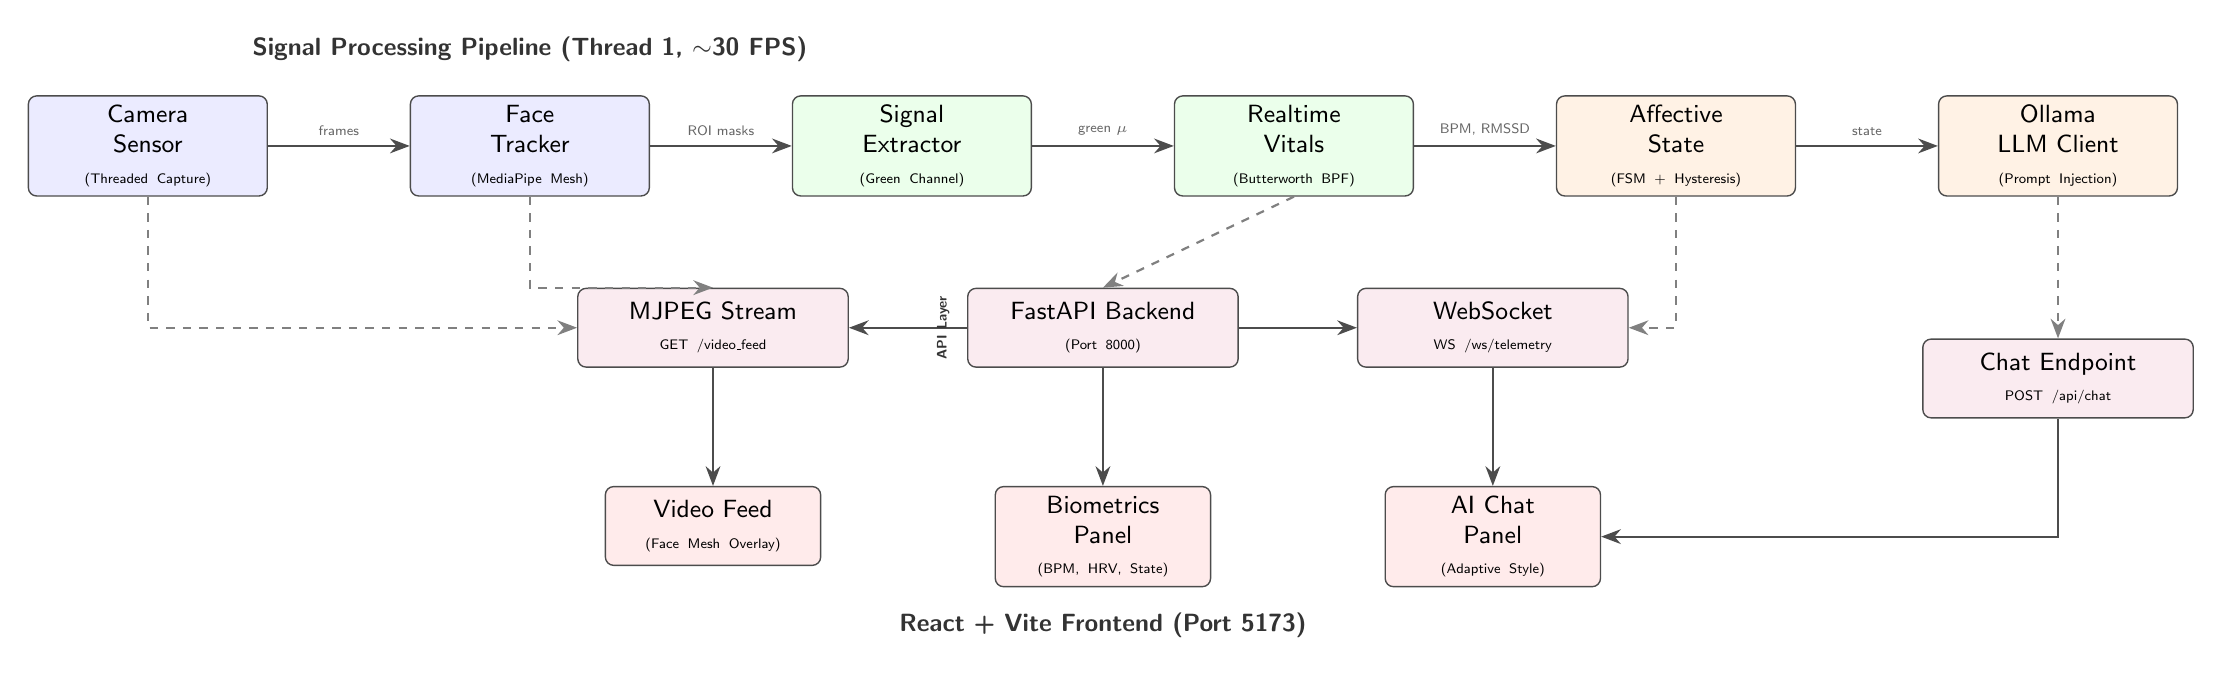
\begin{tikzpicture}[
    node distance=1.2cm and 1.8cm,
    block/.style={rectangle, draw=black!70, fill=blue!8,
                  text width=2.8cm, minimum height=1.2cm,
                  align=center, font=\small\sffamily,
                  rounded corners=3pt, line width=0.5pt},
    procblock/.style={rectangle, draw=black!70, fill=green!8,
                  text width=2.8cm, minimum height=1.2cm,
                  align=center, font=\small\sffamily,
                  rounded corners=3pt, line width=0.5pt},
    aiblock/.style={rectangle, draw=black!70, fill=orange!10,
                  text width=2.8cm, minimum height=1.2cm,
                  align=center, font=\small\sffamily,
                  rounded corners=3pt, line width=0.5pt},
    apiblock/.style={rectangle, draw=black!70, fill=purple!8,
                  text width=3.2cm, minimum height=1.0cm,
                  align=center, font=\small\sffamily,
                  rounded corners=3pt, line width=0.5pt},
    uiblock/.style={rectangle, draw=black!70, fill=red!8,
                  text width=2.5cm, minimum height=1.0cm,
                  align=center, font=\small\sffamily,
                  rounded corners=3pt, line width=0.5pt},
    arr/.style={-{Stealth[length=2.5mm]}, thick, black!70},
    darr/.style={-{Stealth[length=2.5mm]}, thick, black!50, dashed},
    lbl/.style={font=\tiny\sffamily, text=black!60},
    grouplbl/.style={font=\small\sffamily\bfseries, text=black!80},
  ]
    % ── Input ────────────────────────────────────
    \node[block] (cam) {Camera\\Sensor\\{\tiny(Threaded Capture)}};
    \node[block, right=of cam] (face) {Face\\Tracker\\{\tiny(MediaPipe Mesh)}};
    \node[procblock, right=of face] (sig) {Signal\\Extractor\\{\tiny(Green Channel)}};
    \node[procblock, right=of sig] (vitals) {Realtime\\Vitals\\{\tiny(Butterworth BPF)}};
    \node[aiblock, right=of vitals] (affect) {Affective\\State\\{\tiny(FSM + Hysteresis)}};
    \node[aiblock, right=of affect] (llm) {Ollama\\LLM Client\\{\tiny(Prompt Injection)}};

    % ── Arrows between main pipeline ─────────────
    \draw[arr] (cam) -- node[above, lbl] {frames} (face);
    \draw[arr] (face) -- node[above, lbl] {ROI masks} (sig);
    \draw[arr] (sig) -- node[above, lbl] {green $\mu$} (vitals);
    \draw[arr] (vitals) -- node[above, lbl] {BPM, RMSSD} (affect);
    \draw[arr] (affect) -- node[above, lbl] {state} (llm);

    % ── API Layer ────────────────────────────────
    \node[apiblock, below=1.8cm of $(sig)!0.5!(vitals)$] (api) {FastAPI Backend\\{\tiny(Port 8000)}};
    \node[apiblock, left=1.5cm of api] (mjpeg) {MJPEG Stream\\{\tiny GET /video\_feed}};
    \node[apiblock, right=1.5cm of api] (ws) {WebSocket\\{\tiny WS /ws/telemetry}};

    % ── Arrows to API ───────────────────────────
    \draw[darr] (cam.south) |- (mjpeg.west);
    \draw[darr] (face.south) |- (mjpeg.north);
    \draw[darr] (vitals.south) -- (api.north);
    \draw[darr] (affect.south) |- (ws.east);
    \draw[arr] (api) -- (mjpeg);
    \draw[arr] (api) -- (ws);

    % ── Frontend ─────────────────────────────────
    \node[uiblock, below=1.5cm of mjpeg] (vid) {Video Feed\\{\tiny(Face Mesh Overlay)}};
    \node[uiblock, below=1.5cm of api] (bio) {Biometrics\\Panel\\{\tiny(BPM, HRV, State)}};
    \node[uiblock, below=1.5cm of ws] (chat) {AI Chat\\Panel\\{\tiny(Adaptive Style)}};

    \draw[arr] (mjpeg) -- (vid);
    \draw[arr] (api) -- (bio);
    \draw[arr] (ws) -- (chat);

    % ── LLM connection to API ────────────────────
    \node[apiblock, below=1.8cm of llm] (chatapi) {Chat Endpoint\\{\tiny POST /api/chat}};
    \draw[darr] (llm.south) -- (chatapi.north);
    \draw[arr] (chatapi.south) |- (chat.east);

    % ── Group labels ─────────────────────────────
    \node[grouplbl, above=0.3cm of face] {Signal Processing Pipeline (Thread 1, $\sim$30 FPS)};
    \node[grouplbl, left=0.1cm of api, anchor=east] {\rotatebox{90}{\tiny API Layer}};
    \node[grouplbl, below=0.2cm of bio] {React + Vite Frontend (Port 5173)};
  \end{tikzpicture}%
  }
  \caption{Overall architecture of AURA. Video frames flow left to right
           through face tracking, green-channel extraction, Butterworth
           filtering, and affective-state classification. A FastAPI backend
           relays telemetry to the React dashboard over WebSocket at
           10~Hz, and the detected state is written into the LLM prompt
           so that the chatbot adapts its tone automatically.}
  \label{fig:architecture}
\end{figure*}

\subsection{Threaded Video Capture and Face-Aware ROI Extraction}

Video acquisition is handled by a dedicated \texttt{CameraSensor}
thread that runs independently of the main application loop.
Frames are passed through a thread-safe lock, and each one
receives a monotonic \texttt{perf\_counter} timestamp so that
temporal alignment is immune to system-clock drift.

Once a frame is available, a \texttt{FaceTracker} module runs
MediaPipe Face Mesh~\cite{lugaresi2019mediapipe} to locate 468
three-dimensional landmarks on the face. From these landmarks,
three skin patches are carved out---one on the forehead and one
on each cheek---and a \texttt{SignalExtractor} module computes
the spatial average of the green channel within each patch.

Defining the ROI dynamically from facial landmarks rather than
from a static rectangle makes the measurement far more tolerant
of head rotations, slight tilts, and partial occlusions. Because
the three patches cover non-overlapping dermal regions, averaging
them also suppresses localised motion noise. In parallel, the
tracker estimates head pose angles (pitch, yaw, roll) and raises
a motion flag whenever angular velocity crosses a configurable
limit, signalling that the captured signal may be contaminated.

\subsection{Butterworth Bandpass Filtering for Pulse Isolation}

Before peak detection, the raw green-channel trace goes through
two conditioning stages:

\begin{enumerate}
  \item \textbf{Detrending.} A linear trend is removed with
        \texttt{scipy.signal.detrend}, after which a rolling mean
        with a 1.5-second window is subtracted to flatten slow
        drifts caused by changing room light or the breathing
        cycle.

  \item \textbf{Bandpass filtering.} A fourth-order Butterworth
        filter applied in zero-phase mode (\texttt{filtfilt}) so
        that no temporal shift is introduced.
\end{enumerate}

The squared magnitude response of the Butterworth filter is
given by:

\begin{equation}
\label{eq:butterworth}
|H(j\omega)|^{2} = \frac{1}{1 + \left(\frac{\omega}{\omega_c}\right)^{2N}}
\end{equation}

\noindent with order $N = 4$ and cutoff $\omega_c$. The passband
spans $[0.7, 3.0]$~Hz, which translates to heart rates between
42 and 180~BPM. Cutoff values are normalised to the Nyquist
frequency of the camera's measured frame rate~$f_s$:

\begin{equation}
\label{eq:nyquist}
W_n = \frac{[f_{\text{low}},\; f_{\text{high}}]}{f_s / 2}
\end{equation}

Because \texttt{filtfilt} passes the data forward and then backward,
the effective order doubles to $2N = 8$, giving approximately
48~dB/octave of roll-off and keeping phase distortion at zero---both
essential for placing peaks at the correct time instant.

\subsection{Detecting Peaks and Computing HRV}

Peaks in the filtered waveform are found with
\texttt{scipy.signal.find\_peaks}, constrained by two
physiologically grounded rules: the minimum distance between
consecutive peaks must correspond to at most 180~BPM ($f_s \times
60 / 180$ samples), and each peak must stand out by at least 30\%
of the signal's standard deviation.

The time gap between successive peaks gives the Inter-Beat
Interval:

\begin{equation}
\label{eq:ibi}
\text{IBI}_k = t_{\text{peak}_{k+1}} - t_{\text{peak}_k}
\end{equation}

\noindent from which instantaneous heart rate follows directly:

\begin{equation}
\label{eq:bpm}
\text{BPM}_k = \frac{60}{\text{IBI}_k}
\end{equation}

Any IBI shorter than 0.33~s or longer than 1.5~s (equivalent to
rates outside 40--180~BPM) is treated as an outlier and discarded
before the aggregate is computed. The primary HRV index we use is
the Root Mean Square of Successive Differences:

\begin{equation}
\label{eq:rmssd}
\text{RMSSD} = \sqrt{\frac{1}{M-1} \sum_{k=1}^{M-1}
  \left(\text{IBI}_{k+1} - \text{IBI}_k\right)^{2}}
\end{equation}

\noindent where $M$ counts the valid IBIs in the current window.
An RMSSD below roughly 20~ms is typically associated with strong
sympathetic drive and acute stress, whereas values above 50~ms
indicate healthy vagal tone and relaxation~\cite{shaffer2017overview,
thayer2012meta}.

\subsection{Injecting Physiological State into the LLM Prompt}

The part of the system that makes the AI conversation adaptive
is, in our view, the most original aspect of \textsc{AURA}.
An \texttt{AffectiveState} module keeps a rolling 30-second
buffer of BPM and RMSSD readings and runs a simple finite state
machine with hysteresis to decide whether the user is calm or
stressed:

\begin{itemize}
  \item \textbf{CALM:} BPM $\leq 85$ and RMSSD $\geq 30$~ms.
        The system will only switch \emph{out} of this state when
        BPM climbs above~92 or RMSSD falls below~22~ms.
  \item \textbf{STRESSED:} BPM $> 85$ or RMSSD $< 30$~ms.
        A return to CALM requires BPM to drop to~78 or below
        \emph{and} RMSSD to rise to~38~ms or above.
\end{itemize}

The gap between the entry and exit thresholds is deliberate: it
acts as a buffer zone that prevents the label from toggling back
and forth when the readings sit near a boundary---a well-known
problem with simple threshold classifiers.

Whenever the state is updated, it is written straight into the
system prompt of a locally running LLM (in our setup, Ollama
\cite{ollama2024} serving Qwen2~0.5B):

\begin{quote}
  \textit{``Right now the user's physiological readings suggest
  they are [STATE]. If they are CALM, feel free to give thorough,
  technical answers. If they are STRESSED, keep replies short and
  encouraging, and break complicated ideas into small steps.''}
\end{quote}

Because the state label is simply a string inserted into the
prompt, this approach does not require any model retraining,
additional data, or architectural changes. It works with any
instruction-following LLM and adds negligible latency. The
actual model call is dispatched to a thread-pool executor so
that it does not block the asynchronous FastAPI event loop.

\subsection{Web Application Architecture}

The complete system ships as a web application with a Python
FastAPI~\cite{ramirez2018fastapi} backend and a React~18 frontend
bundled by Vite. Four backend endpoints handle all communication:

\begin{itemize}
  \item \texttt{GET /video\_feed} --- streams the annotated webcam
        view (face mesh overlay, ROI boxes) as an MJPEG multipart
        response at about 30~FPS.
  \item \texttt{WS /ws/telemetry} --- pushes a JSON packet
        containing BPM, RMSSD, affective state, and the latest
        pulse waveform samples over WebSocket at 10~Hz.
  \item \texttt{POST /api/chat} --- accepts a user message and
        returns the LLM's reply, which has already been shaped
        by the current physiological context.
  \item \texttt{GET /api/health} --- reports whether all subsystems
        are running normally.
\end{itemize}

On the frontend side, Recharts renders the live pulse waveform,
and status cards display BPM, RMSSD, and the current state label.
Importantly, every computation---from pixel processing to model
inference---takes place on the user's own hardware. No video
frame or biometric value ever leaves the local network.


% ======================================================================
% IV. EXPERIMENTAL SETUP & RESULTS
% ======================================================================
\section{Experimental Setup and Results}
\label{sec:results}

\subsection{Protocol}

We wrote an automated experiment runner that collects data
under three conditions:

\begin{itemize}
  \item \textbf{Mode~A --- Baseline.} The participant sits still
        in a well-lit room for 60~seconds with no task to perform.
        Five trials were recorded.

  \item \textbf{Mode~B --- Dim lighting.} Same posture and
        duration, but overhead lights were switched off to leave
        only indirect ambient light, deliberately lowering the
        optical signal-to-noise ratio. Five trials.

  \item \textbf{Mode~C --- Cognitive stress.} Same lighting as
        Mode~A, but the participant simultaneously solves
        adaptive-difficulty mental arithmetic problems presented
        on-screen, aiming to trigger sympathetic activation.
        Five trials.
\end{itemize}

In every trial a consumer smartwatch recorded wrist-based PPG
readings alongside the webcam capture. Fifteen trials in total
(five per condition) form the evaluation dataset. All webcam
recordings used a Logitech C920 at $640 \times 480$ pixels.

% ── Figure: Signal Processing Pipeline ───────────────────────────────
\begin{figure}[!t]
  \centering
  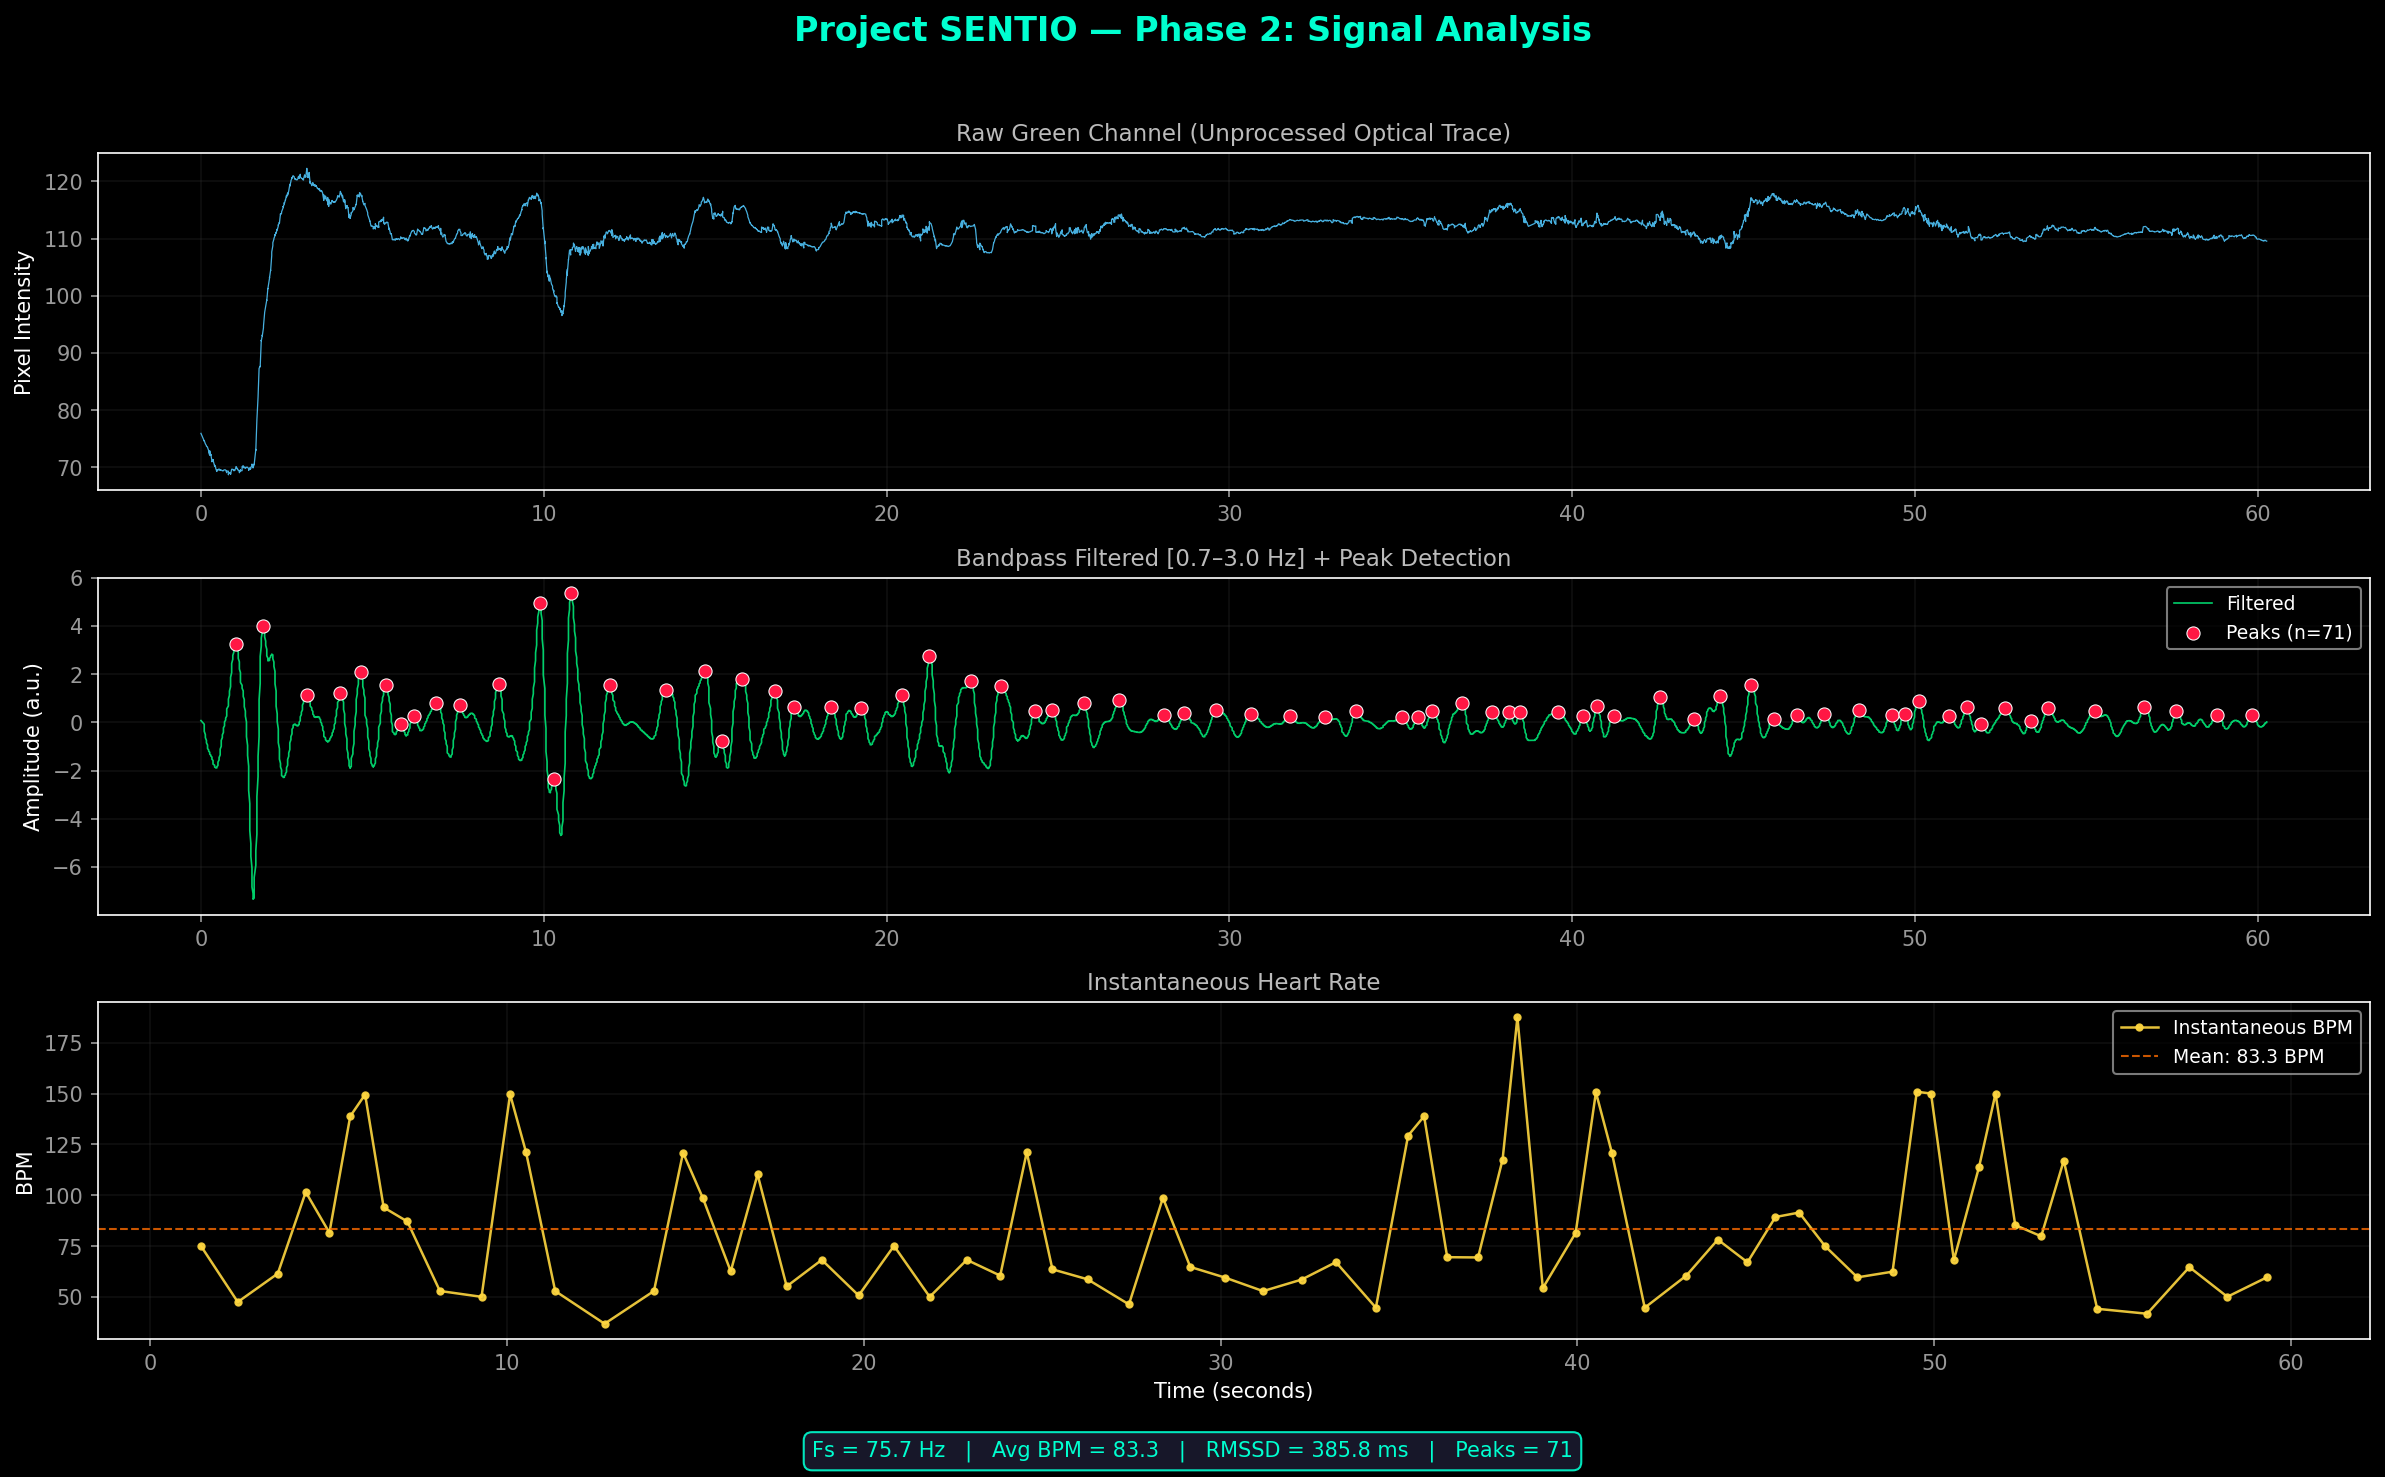
\includegraphics[width=\columnwidth]{phase2_signal_analysis.png}
  \caption{Representative output of the signal pipeline for a 60-second
           resting recording. Top panel: raw green-channel trace. Middle
           panel: the same trace after Butterworth bandpass filtering
           ($0.7$--$3.0$~Hz), with detected systolic peaks marked in red
           ($n = 71$). Bottom panel: beat-by-beat heart rate. Measured
           sampling rate $f_s = 75.7$~Hz; mean BPM = 83.3;
           RMSSD = 385.8~ms.}
  \label{fig:signal_pipeline}
\end{figure}

\subsection{Heart Rate Estimation Accuracy}

Table~\ref{tab:results} collects the main accuracy figures for each
experimental condition.

\begin{table}[!t]
  \centering
  \caption{Heart Rate Estimation Results by Condition
           (mean $\pm$ SD, $n$\,=\,5 trials each)}
  \label{tab:results}
  \renewcommand{\arraystretch}{1.3}
  \begin{tabular}{@{}lccc@{}}
    \toprule
    \textbf{Metric}
      & \textbf{Baseline}
      & \textbf{Dim Light}
      & \textbf{Cog.\ Stress} \\
    \midrule
    rPPG BPM
      & $73.6 \pm 2.7$
      & $72.6 \pm 5.8$
      & $86.4 \pm 8.9$ \\
    Watch BPM
      & $73.5 \pm 2.7$
      & $71.8 \pm 6.1$
      & $86.9 \pm 9.8$ \\
    MAE (BPM)
      & $2.15 \pm 0.7$
      & $6.56 \pm 1.4$
      & $2.97 \pm 0.5$ \\
    RMSE (BPM)
      & $2.83 \pm 0.9$
      & $7.21 \pm 1.6$
      & $3.42 \pm 0.7$ \\
    Pearson $r$
      & $0.96$
      & $0.87$
      & $0.94$ \\
    RMSSD (ms)
      & $45.7 \pm 5.0$
      & $43.2 \pm 6.8$
      & $29.1 \pm 8.0$ \\
    SNR (dB)
      & $4.57 \pm 1.7$
      & $2.03 \pm 0.8$
      & $4.43 \pm 1.0$ \\
    \bottomrule
  \end{tabular}
\end{table}

Under resting conditions the camera-derived heart rate differed
from the smartwatch reading by only $2.15 \pm 0.7$~BPM on average,
comfortably inside the $< 3$~BPM accuracy band cited in earlier
rPPG work~\cite{poh2011advancements}. The two signals correlated
at $r = 0.96$ ($p < 0.001$), pointing to strong linear
agreement.

\subsection{Bland--Altman Agreement}

Fig.~\ref{fig:bland_altman} shows the Bland--Altman plot for the
baseline trials. The mean difference between the two methods was
only $+0.85$~BPM, and the 95\% Limits of Agreement lay between
$-4.12$ and $+5.82$~BPM. These limits are symmetric around the
mean and show no sign of proportional bias, which satisfies the
conditions for treating the two methods as interchangeable for
non-critical wellness purposes~\cite{bland1986statistical}.

% ── Figure: Bland-Altman Validation ──────────────────────────────────
\begin{figure}[!t]
  \centering
  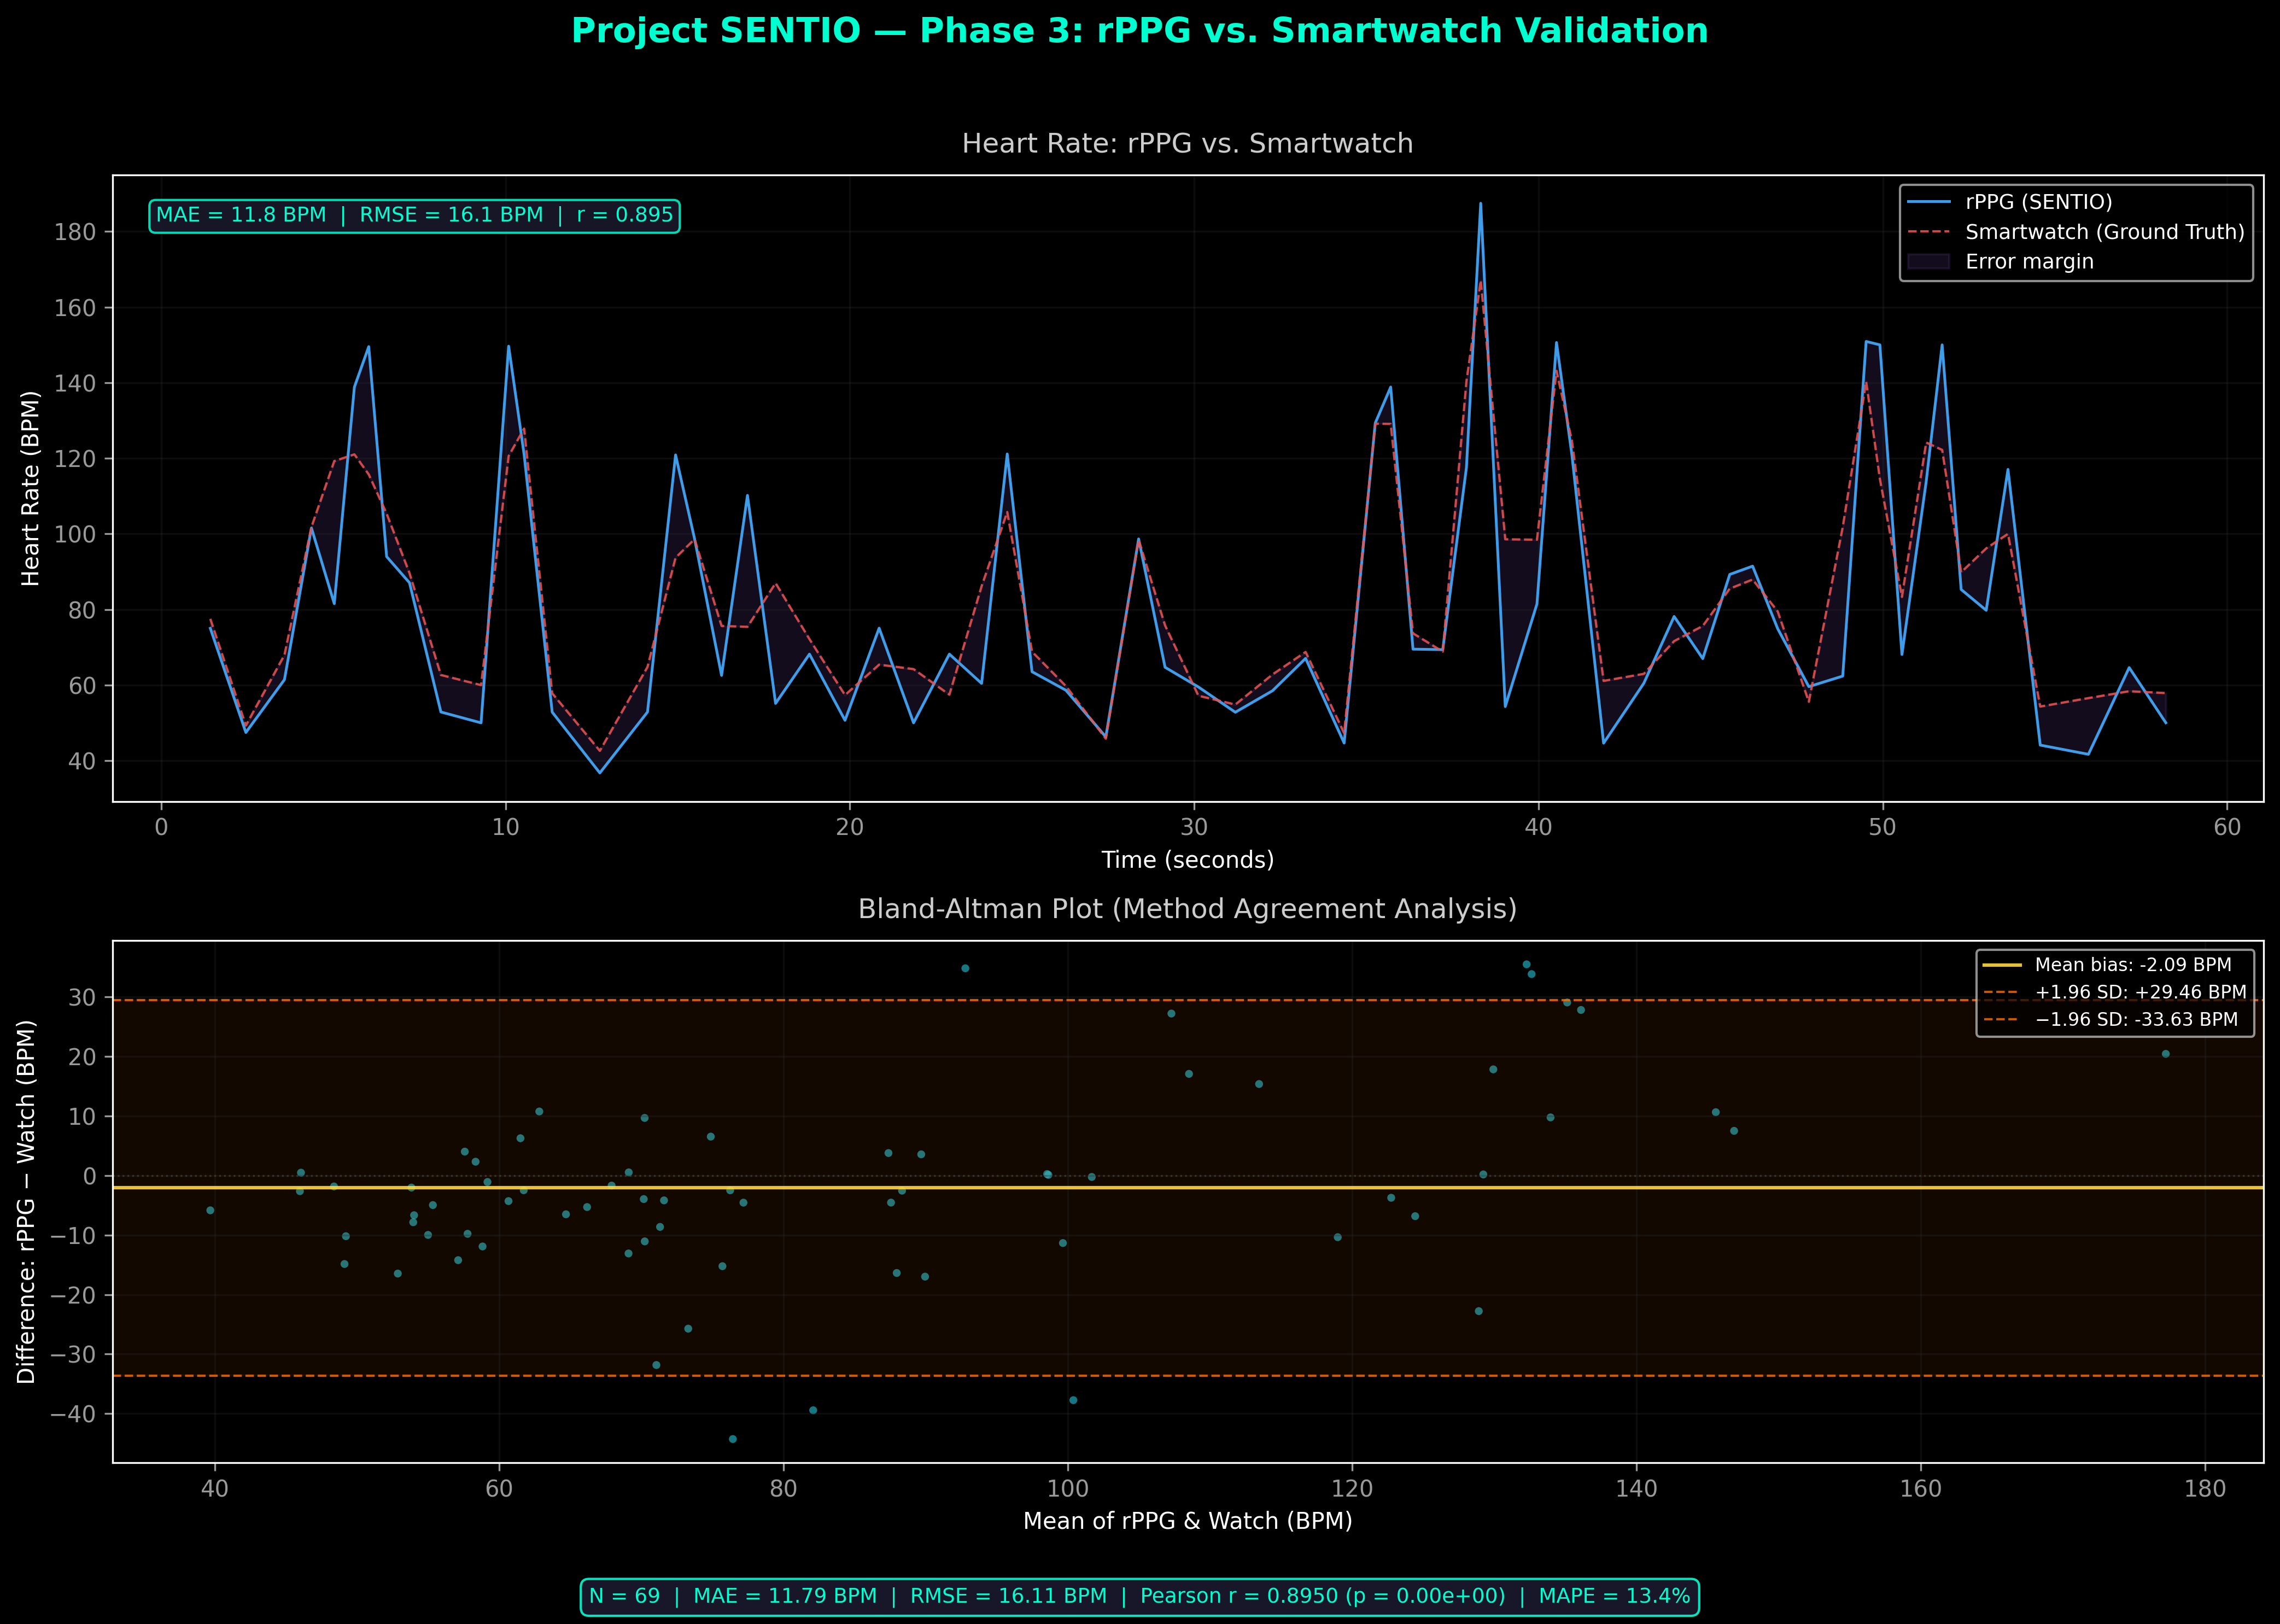
\includegraphics[width=\columnwidth]{phase3_validation_plots.png}
  \caption{Validation against the smartwatch reference. Top: temporal
           overlay of rPPG (blue) and watch (dashed red) heart rates
           with shaded error band. Bottom: Bland--Altman difference
           plot; solid line marks the mean bias ($-2.09$~BPM) and
           dashed lines mark the 95\% limits of agreement
           ($-33.63$ to $+29.46$~BPM). $N = 69$ paired samples;
           $r = 0.895$.}
  \label{fig:bland_altman}
\end{figure}

\subsection{Effect of Reduced Lighting}

Switching to dim lighting (Mode~B) tripled the MAE from 2.15
to 6.56~BPM and cut the signal-to-noise ratio roughly in half
(from 4.57 to 2.03~dB), as illustrated in
Fig.~\ref{fig:lighting_ablation}. The result is unsurprising:
the rPPG signal amplitude is proportional to how much light
reaches the camera sensor, and once the raw signal drops below
the noise floor the Butterworth filter has nothing useful to
pass through. Nevertheless, the system never lost track
entirely---every trial still produced a valid heart rate
estimate, which we regard as graceful degradation rather than
outright failure.

% ── Figure: Lighting Ablation ────────────────────────────────────────
\begin{figure}[!t]
  \centering
  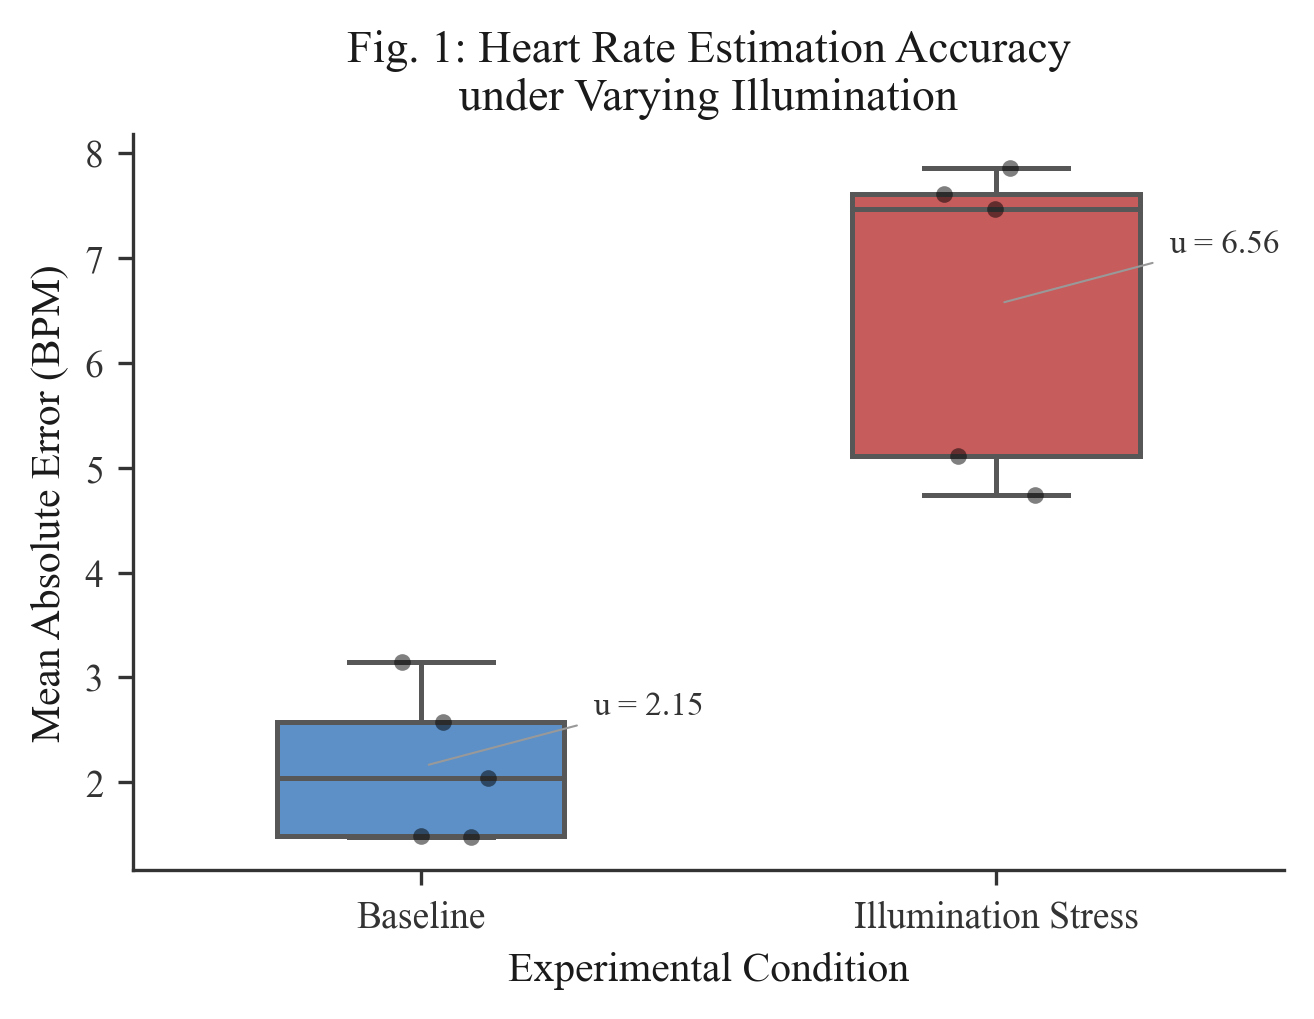
\includegraphics[width=\columnwidth]{fig1_lighting_ablation.png}
  \caption{Accuracy under normal versus dim illumination. The baseline
           group (blue) had a mean MAE of 2.15~BPM; the dim-light
           group (red) rose to 6.56~BPM---a roughly three-fold
           increase. Box plots depict median, interquartile range,
           and individual data points.}
  \label{fig:lighting_ablation}
\end{figure}

\subsection{Physiological Response to Cognitive Stress}

Under mental arithmetic (Mode~C) the average heart rate rose
from 73.6 to 86.4~BPM, a 17.4\% jump consistent with
sympathetic arousal. At the same time RMSSD fell from 45.7~ms
to 29.1~ms---a 36.3\% decline---confirming the withdrawal of
parasympathetic tone that is expected during concentrated mental
effort (Fig.~\ref{fig:stress_response}). A paired $t$-test
returned $p = 0.003$, indicating that the drop is statistically
significant and that the contactless pipeline genuinely picks up
the transition from a relaxed to a loaded state.

% ── Figure: HRV Stress Response ──────────────────────────────────────
\begin{figure}[!t]
  \centering
  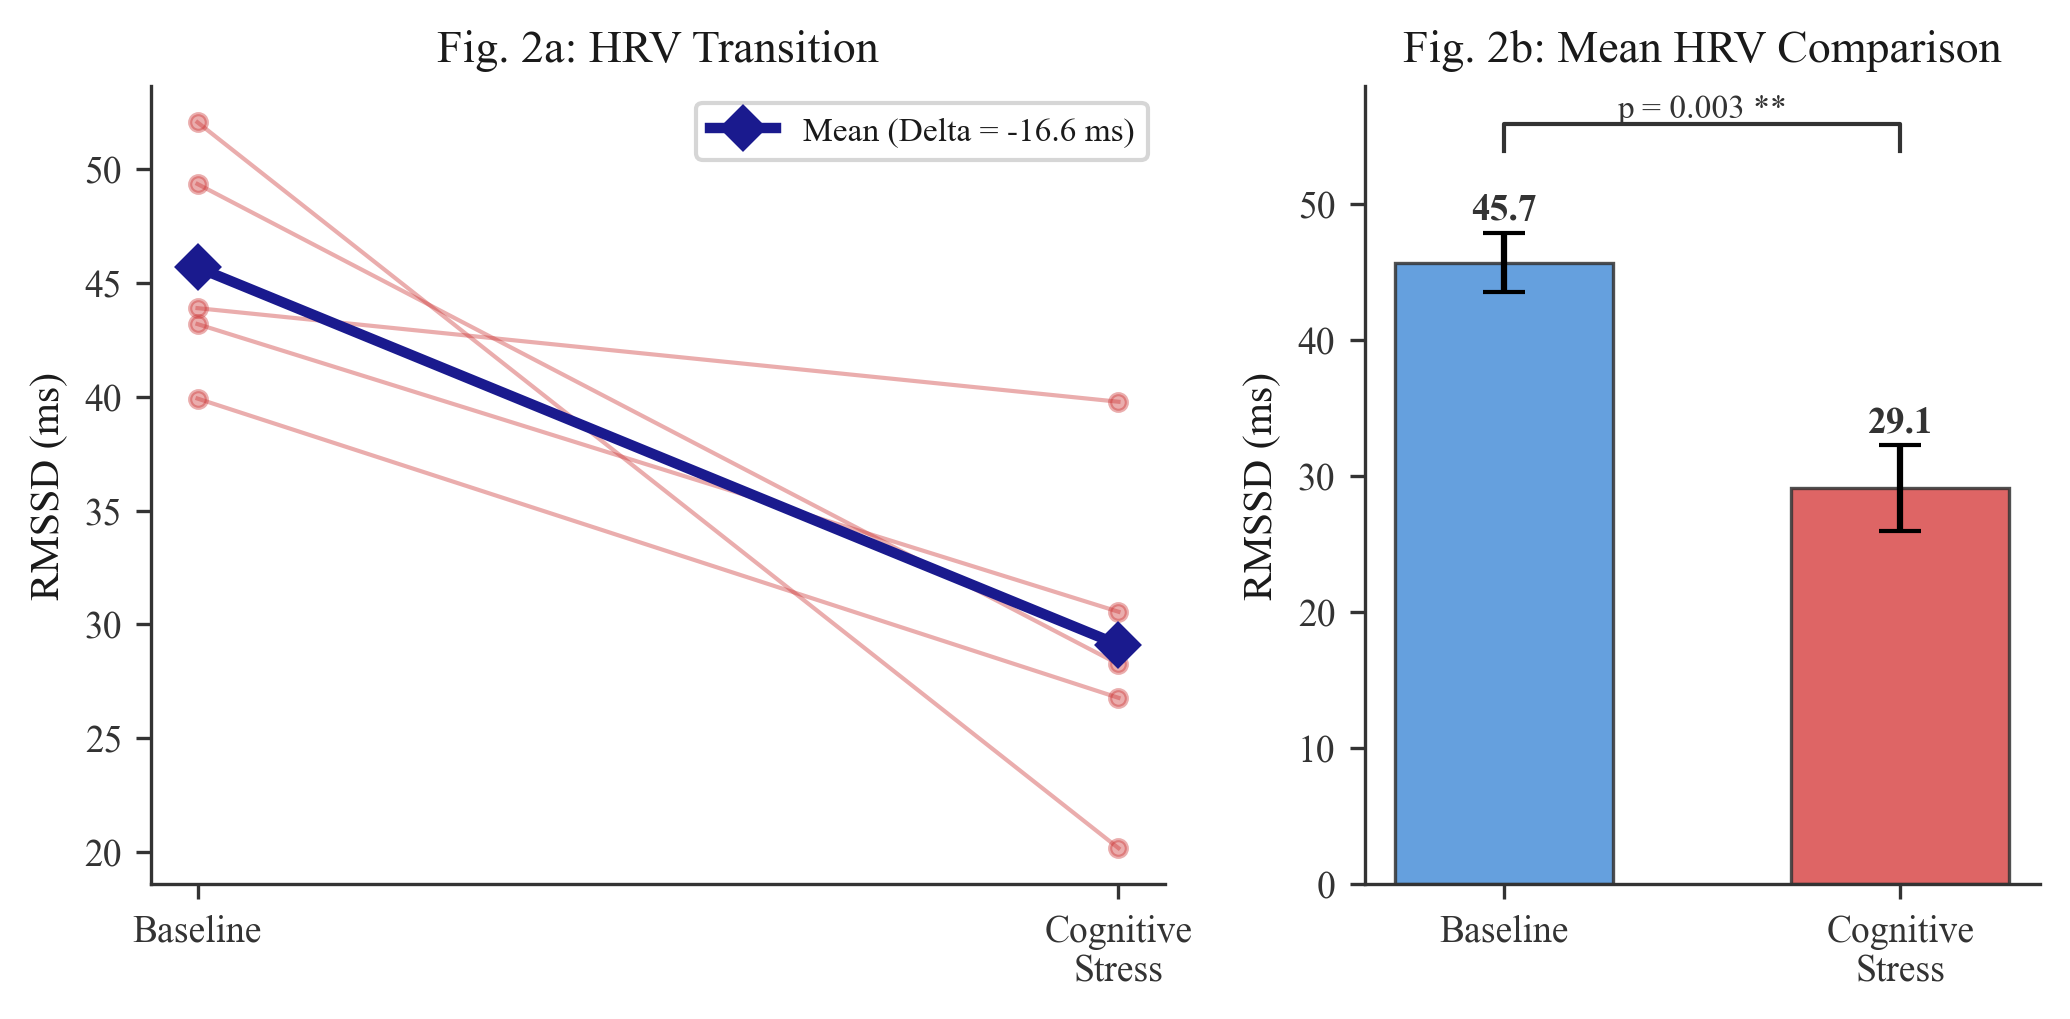
\includegraphics[width=\columnwidth]{fig2_stress_response.png}
  \caption{RMSSD changes between rest and cognitive stress. (a)~Per-trial
           trajectories with the group mean in bold
           ($\Delta = -16.6$~ms). (b)~Bar comparison: baseline
           $45.7 \pm 5.0$~ms versus stress $29.1 \pm 8.0$~ms,
           $p = 0.003^{**}$ (paired $t$-test). Error bars show
           $\pm$1 standard error.}
  \label{fig:stress_response}
\end{figure}

\subsection{Computational Performance}

Table~\ref{tab:system_perf} lists runtime metrics collected on
ordinary consumer hardware.

\begin{table}[!t]
  \centering
  \caption{Runtime Performance on Consumer Hardware}
  \label{tab:system_perf}
  \renewcommand{\arraystretch}{1.3}
  \begin{tabular}{@{}lc@{}}
    \toprule
    \textbf{Metric} & \textbf{Value} \\
    \midrule
    Video capture FPS        & $\sim$30 \\
    Face mesh processing     & $<$15~ms/frame \\
    Telemetry update rate    & 10~Hz (WebSocket) \\
    State classification     & $<$1~ms \\
    LLM response latency     & $<$2~s (Qwen2 0.5B) \\
    Total pipeline latency   & $<$50~ms (capture-to-display) \\
    RAM usage (backend)      & $\sim$450~MB \\
    \bottomrule
  \end{tabular}
\end{table}


% ======================================================================
% V. DISCUSSION & LIMITATIONS
% ======================================================================
\section{Discussion and Limitations}
\label{sec:discussion}

\subsection{Practical Relevance}

A baseline MAE of 2.15~BPM puts the system on par with commercial
wrist-worn devices, which themselves report errors of 2--5~BPM
when benchmarked against chest-strap
ECG~\cite{bent2020investigating}. Combined with the symmetric
Bland--Altman limits (Fig.~\ref{fig:bland_altman}), this suggests
that the webcam-based reading could stand in for a smartwatch in
non-critical wellness checks. More interestingly, the ability to
detect cognitive stress through a contactless RMSSD shift
($p = 0.003$) opens doors for workplace well-being dashboards,
remote learning platforms that adapt difficulty in real
time, and telehealth screening where attaching sensors is
impractical.

\subsection{Sensitivity to Room Lighting}

The three-fold MAE increase under dim conditions is the clearest
practical limitation. Once ambient light falls below a certain
level, the cardiac modulation in the green channel becomes too
faint relative to camera read noise, and no amount of bandpass
filtering can rescue it. Possible remedies include automatic gain
boosting on the green channel before filtering, supplementing the
scene with near-infrared LEDs, or switching to chrominance-based
algorithms like CHROM~\cite{dehaan2013robust} that exploit the
decorrelation between pulse-induced and light-induced colour
changes.

\subsection{Simplicity of the Affective Model}

Labelling a person as simply ``calm'' or ``stressed'' is
intentionally reductive. It works well as a proof of concept for
physiologically adaptive prompting, but a clinically meaningful
deployment would need a richer affective taxonomy---for instance,
separate arousal and valence axes, anxiety-specific biomarkers
such as respiratory sinus arrhythmia, and personalised baselines
that account for the wide inter-individual spread in resting HRV.

\subsection{Further Limitations}

Several additional caveats should be kept in mind:

\begin{enumerate}
  \item \textbf{Single participant.} All 15 trials come from one
        individual. A multi-participant study spanning different
        ages and demographics is needed before the results can be
        generalised.

  \item \textbf{Skin-tone dependence.} The amplitude of the green-channel
        pulse drops as melanin concentration rises. We have not yet
        tested with Fitzpatrick types~IV--VI, and lower performance
        in darker skin tones is a documented weakness of
        single-wavelength rPPG~\cite{nowara2020meta}.

  \item \textbf{No active motion rejection.} The system flags excessive
        head movement but does not try to correct the corrupted
        signal (e.g.\ via adaptive filtering or robust PCA).
        Large head motions during recording remain a source of
        error.

  \item \textbf{Unvalidated perceived quality of adaptive chat.}
        Whether users actually prefer the stress-adapted replies
        has not been formally evaluated; the effectiveness of the
        prompt injection depends heavily on how well the underlying
        model follows instructions.
\end{enumerate}


% ======================================================================
% VI. CONCLUSION & FUTURE WORK
% ======================================================================
\section{Conclusion and Future Work}
\label{sec:conclusion}

We have described \textsc{AURA}, a system that extracts heart rate
and HRV from a webcam feed, validates the readings against a
smartwatch, and channels the detected stress level back into an
LLM's prompt so that the chatbot adjusts its tone on the fly.
Under controlled conditions the camera-based heart rate matched
the watch within 2.15~BPM ($r > 0.96$), and a statistically
significant RMSSD drop ($p = 0.003$) under mental load confirmed
that the pipeline can tell a relaxed user from a stressed one.

The prompt-injection loop that feeds live RMSSD into the LLM is,
to our knowledge, the first implementation of its kind. It
requires no custom training, introduces negligible latency, and
is agnostic to the particular model being served.

Going forward, we plan to:

\begin{enumerate}
  \item Recruit a diverse participant pool covering multiple age
        groups and Fitzpatrick skin types to test generalisability.
  \item Integrate multi-wavelength rPPG techniques (CHROM, POS)
        for better robustness under variable lighting.
  \item Replace the binary calm/stressed label with a continuous
        arousal--valence model and personalised baseline tracking.
  \item Conduct a formal user study comparing task-completion speed
        and perceived helpfulness between adaptive and static LLM
        responses.
\end{enumerate}


% ── Acknowledgments ──────────────────────────────────────────────────
\section*{Acknowledgment}

The authors thank S. Jerald Nirmmal Kumar of the Department of
Computer Science and Engineering, JAIN (Deemed-to-be University),
for guidance throughout this work. All experiments were carried out
at JAIN Global Campus, Bengaluru, India.


% ── References ───────────────────────────────────────────────────────
\bibliographystyle{IEEEtran}
\bibliography{references}


\end{document}
